% questions.tex —— 1977 年·广西卷（文科） · 题目内容片段（无答案）
% 由 tools/generate_projects.py 依来源总账自 1977/1977_数学真题_广西文_试题.md 生成，勿手改（改源 MD 后重跑）


\gkpart{广西壮族自治区（文科）}

\begin{gktip}
\textbf{来源说明}：本题面依据固定源 PDF《1977广西文》第 1—5 页逐题转录（第 1—4 页带书页码 137—140，第 5 页未见书页码）。固定源是题面与解答连排的书籍材料：每题题面后紧跟「解」「证明」「答」，并非空白试卷；本文只转录题面，配套答案与解析由本库对照源解答独立复算推导，\textbf{非官方标准答案}。原卷按大题「一、」至「五、」编号：第一大题带总头「（每小题6分，本题满分30分）」下辖 5 个小题，第二至第五大题各为单题，分值分别为 16 分、17 分、15 分、22 分，全卷合计 100 分；本库将大题重排为连续题号 1—5，第一大题的 5 个小题统一为（1）—（5）小问格式，未增删题干。原卷第二大题与第五大题各附一幅示意图，LaTeX 版按源图重绘。无附加题、参考题。
\end{gktip}

\par\medskip

\begin{question}
\gkti{1}\textbf{（30 分）} 

（1） 计算 $5\frac{3}{4}-2\left[\left(\frac{1}{2}\right)^2-3\times\frac{3}{4}\right]\div\frac{2}{5}$。

（2） 分解 $x^3-5x^2+4x$ 的因式。

（3） 化简 $\dfrac{1}{\sin^2\alpha}-\operatorname{ctg}^2\alpha$。

（4） 计算 $\operatorname{ctg}135^\circ+\cos(-60^\circ)-\operatorname{tg}^260^\circ+\sin30^\circ$。

（5） 不查表求 $\lg\dfrac{3}{7}+\lg70-\lg3$ 的值。

\Needspace{0.4\textheight}
\end{question}
\begin{question}
\gkti{2}\textbf{（16 分）} $P$ 是圆外一点，过 $P$ 作两条直线，一条交圆于 $C$、$A$ 两点，一条交圆于 $D$、$B$ 两点，求证 $PA\cdot PC=PB\cdot PD$。

\begin{gktip}
原源 PDF 第 3 页附有圆与两条割线、两条虚线弦的示意图；LaTeX 版按源图重绘。
\end{gktip}
\nopagebreak[4]
\begin{center}% 1977 年广西卷第 2 题：圆外一点 P 的两条割线 P-D-B、P-C-A 与两条虚线弦 AD、BC（按源卷第 3 页布局）
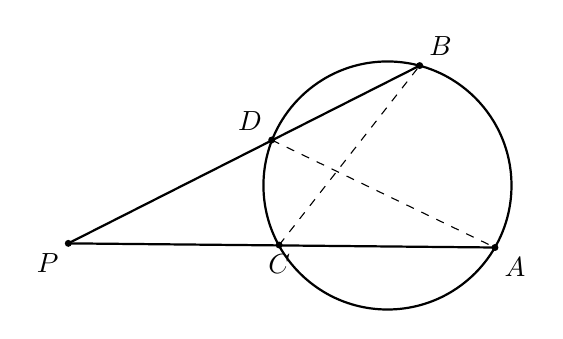
\begin{tikzpicture}[scale=1.05]
  % 圆
  \draw[thick] (0,0) circle (1.5);
  % 割线端点与圆上点（坐标手算：D、B、C、A 均在圆上，P 在圆外）
  \coordinate (P) at (-3.86,-0.70);
  \coordinate (D) at (-1.40,0.55);
  \coordinate (B) at (0.39,1.45);
  \coordinate (C) at (-1.31,-0.72);
  \coordinate (A) at (1.30,-0.75);
  % 两条割线（整段直画，保证共线）
  \draw[thick] (P) -- (B);
  \draw[thick] (P) -- (A);
  % 两条虚线弦
  \draw[dashed] (D) -- (A);
  \draw[dashed] (C) -- (B);
  % 顶点与标注
  \fill (P) circle (1.2pt) node[below left] {$P$};
  \fill (D) circle (1.2pt) node[above left] {$D$};
  \fill (B) circle (1.2pt) node[above right] {$B$};
  \fill (C) circle (1.2pt) node[below] {$C$};
  \fill (A) circle (1.2pt) node[below right] {$A$};
\end{tikzpicture}
\end{center}
\nopagebreak[4]
\end{question}
\begin{question}
\gkti{3}\textbf{（17 分）} $m$ 是什么值的时候，方程

\nopagebreak[4]
\[
3x^2-(4m-1)x+m^2+\frac{3}{4}=0
\]

有相等的两个实数根。

\end{question}
\begin{question}
\gkti{4}\textbf{（15 分）} 波尔多液由胆矾、生石灰和水配制成，已知胆矾和生石灰的重量比是 $1:2$，生石灰和水的重量比是 $1:120$，问配制 $486$ 斤波尔多液需胆矾、生石灰和水各多少斤？

\Needspace{0.4\textheight}
\end{question}
\begin{question}
\gkti{5}\textbf{（22 分）} 已知桥的一孔为抛物线型（如图），跨度 $AB=12$ 米，桥孔高 $PO=4$ 米，建桥时每隔 $2$ 米一个撑梁，求撑梁 $C_1D_1$，$C_2D_2$，$C_3D_3$，$C_4D_4$ 各应取多长？

\begin{gktip}
原源 PDF 第 4 页附有抛物线拱桥直角坐标系示意图；LaTeX 版按源图重绘。
\end{gktip}
\nopagebreak[4]
\begin{center}% 1977 年广西卷第 5 题：抛物线拱桥 x²=−9y，顶点在原点、开口向下，
% 跨度 AB=12 米（A(−6,−4)、B(6,−4)），撑梁 C1D1…C4D4 竖直，桥面线 y=−4（按源卷第 4 页布局）
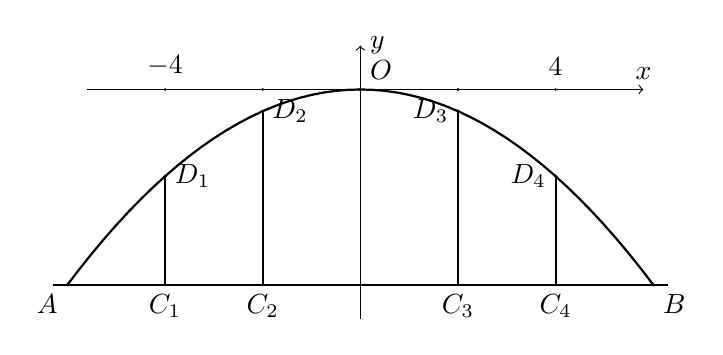
\begin{tikzpicture}[scale=0.62]
  % 坐标轴
  \draw[->] (-5.6,0) -- (5.8,0) node[above] {$x$};
  \draw[->] (0,-4.7) -- (0,0.9) node[right] {$y$};
  \fill (0,0) circle (1.1pt) node[above right] {$O$};
  % 抛物线 y = -x^2/9（顶点在原点，开口向下）
  \draw[thick, domain=-6:6, samples=49] plot (\x, {-\x*\x/9});
  % 桥面线（弦 AB 所在水平线）
  \draw[thick] (-6.3,-4) -- (6.3,-4);
  \fill (-6,-4) circle (1.1pt) node[below left] {$A$};
  \fill (6,-4) circle (1.1pt) node[below right] {$B$};
  % 四根撑梁（x=±2、±4）
  \foreach \i/\xx in {1/-4, 2/-2, 3/2, 4/4} {
    \pgfmathsetmacro{\yy}{-\xx*\xx/9}
    \draw[thick] (\xx,-4) -- (\xx,\yy);
    \fill (\xx,-4) circle (1pt) node[below] {$C_{\i}$};
    \pgfmathtruncatemacro{\side}{\xx>0 ? -1 : 1}
    \ifnum\side<0
      \fill (\xx,\yy) circle (1pt) node[left] {$D_{\i}$};
    \else
      \fill (\xx,\yy) circle (1pt) node[right] {$D_{\i}$};
    \fi
  }
  % x 轴刻度点与标注（−4 与 4）
  \foreach \xx in {-4,-2,2,4} { \fill (\xx,0) circle (0.9pt); }
  \node[above] at (-4,0.08) {$-4$};
  \node[above] at (4,0.08) {$4$};
\end{tikzpicture}
\end{center}
\nopagebreak[4]

\end{question}